\section{Approach}\label{sec:approach}

\sepfootnotecontent{sf:shapeIndexURL}{
   \ifanonymous
      \url{https://anonymous.4open.science/w/shape-index-specification-707E}
   \else
      \url{https://constraintautomaton.github.io/shape-index-specification/}
   \fi
}

\sepfootnotecontent{sf:recursiveShape}{
    In this paper we ignore "inverse constraints" such as
    inverse triple constraint in ShEx 
    %\url{https://shex.io/shex-primer/index.html\#inverse-properties}
    and SHACL Inverse Paths 
    %\url{https://www.w3.org/TR/shacl\#property-path-inverse} 
    to avoid recurse 
    shape schemas~\cite{Corman2019}.
    We only consider shapes that can be transformed into a single \texttt{SELECT} SPARQL query.
}

\sepfootnotecontent{sf:subwebsep}{
   We assume an implicit conversion between the subweb specification and the formalization of reachability criteria.
   Space constraints prevent us from detailing the conversion.
}

\sepfootnotecontent{sf:ssf_project}{
   The paper \citetitle{delva2023} additional material also proposes a script to convert SCHACL shapes into SPARQL queries.
   \url{https://github.com/MaximeJakubowski/ssf_project}
   \rt{This footnote seems unnecessary, since delva2023 is already cited.}
}


In this section, we define our approach by first introducing pruning in LTQP, then explaining the shape index, and finally describing how the shape index is used for pruning in LTQP.
Our approach considers a DKG with subwebs containing shape indexes hosted by data providers. 
By exploiting those indexes, query engines performing LTQP can prune a part of DKG without affecting query results when considering executing the query over the whole network.
Figure~\ref{fig:dkg} presents a schema of our approach and the query execution context.

\begin{figure}
   \centering
   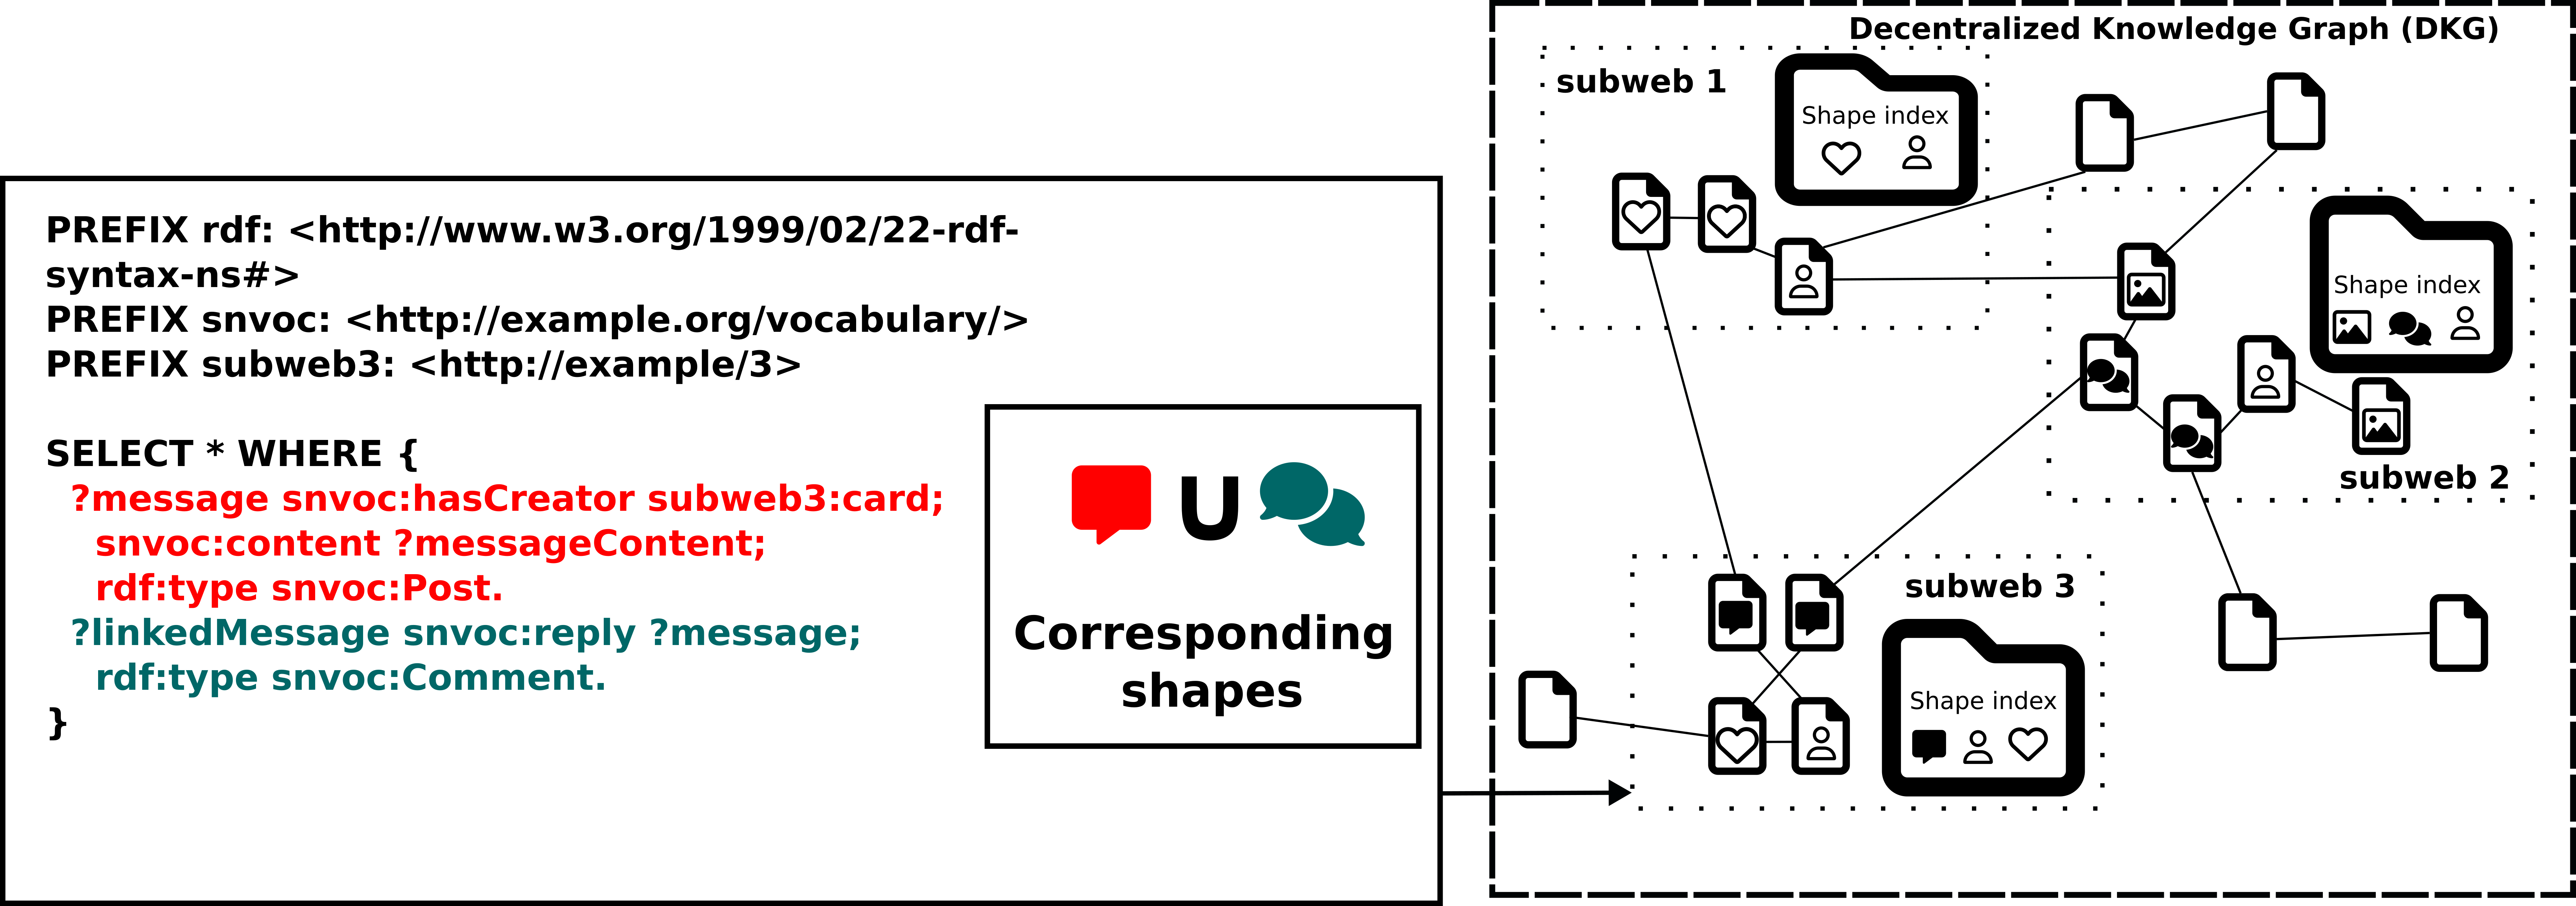
\includegraphics[width=0.45\textwidth]{figure/dkg.png}
   \caption{
      Given that the resources of a DKG are indexed with a shape index, a query engine can dereference a subset of the network.
      The nodes represent RDF resources, while the edges represent IRIs linking one resource to another (see Section \ref{sec:dkg}).
      Each subweb has a shape index that maps shapes, represented by polygons, to RDF resources by embedding the polygon within the node.
      The query engine starts its query at subweb 3, and the relevant query resources in a subweb are identified with a black node.
    }
    \label{fig:dkg}
\end{figure}


\subsection{LTQP Completeness when Pruning}\label{sec:slde}

Our approach of pruning in LTQP focus on ensuring result completeness, assuming traversal completeness is already defined using reachability criteria.
By concentrating on result completeness, we explore strategies to optimize the search space of link traversal queries through pruning of irrelevant sources.
We formalize our approach as follows.
A query is executed over a DKG $G$ formed by the union of all the $g \in r$ in a network $R$.
The query engine has to build a KG $G^{\prime}$ using a reachability $C^{\prime}$ in its internal data store from the $g \in r$ by dereferencing resources in $R$.
We are trying to solve an optimization problem where another query engine builds a KG
$G^{\prime\prime} \subseteq G^{\prime}$
potentially smaller than the one produced with a specific traversal completeness policy
by defining a reachability criterion $C^{\prime\prime}$.
We focus on maintaining the same results completeness, so when using $C^{\prime\prime}$ the following equation must hold

\begin{equation}\label{eq:evalQueryStructuralAssumption}
   [\![ Q ]\!]^{G^{\prime\prime}} = [\![ Q ]\!]^{G^{\prime}}
\end{equation}
for any network $R$.
Because the $g \in G^{\prime}$ can only be acquired from the dereferencing of resources $r \in R$, a smaller $G^\prime$ implies that a lesser number of HTTP requests has been performed to answer a query.
Generaly, query execution is faster with a smaller KG instance.
Additionally, HTTP requests can be slow and unpredictable~\cite{hartig2016walking}, making them a significant factor in overall query execution time. 
Thus, the benefit of reducing the number of HTTP requests is twofold.

To define less selective reachabilities to produce $G^{\prime\prime}$, we propose extending the reachability criteria by formalizing a chain of criteria in a concept called \emph{composite reachability criteria}.
In this form, a reachability criterion $cp_i$ is said to \emph{prune} links, and $cd_i$ is said to \emph{discover} links.
Equation~\ref{eq:cReachabilityCriteria} formalizes a composite reachability criterion $C$.

\begin{equation}\label{eq:cReachabilityCriteria}
   C(t, iri, B) = \bigvee_{cd \in Cd} cd(t, iri, B) \mathrel{\land} \bigwedge_{cp \in Cp} \, cp(t, iri, B)
\end{equation}
where $Cd$ is the set of every $cd_i(t, iri, B)$ and $Cp$ the set of every $cp_i(t, iri, B)$ used by the engine.
This section has introduced our general concept of pruning. 
In the next section, we present our specific shape-based approach using a shape index.

\subsection{Shape Index}

\begin{figure}
   \centering
   \begin{tabular}{c}
      \lstinputlisting[language=sh, basicstyle=\tiny]{code/shape_index.nq}
   \end{tabular}
   \caption{
      An example of a shape index mapping a set of IRI to a profile shape and an IRI to a post shape.
   }
   \label{fig:shapeIndex}
\end{figure}
Pruning in LTQP requires information about the data models of dereferenced sources.
However, obtaining complete, up-to-date, and expensive information for each source in a large decentralized network is unrealistic.
To address this, we propose the concept of the \emph{shape index}. 
We define a shape index is a mapping between sets of RDF documents and RDF data shapes, which describe subweb controlled by a data provider.
When a set of RDF documents is mapped, the associated KG must conform to the shape.
Unlike statistics on triples, shapes are independent of the size of the KG or updates that remain compliant with the shape, making them a more cost-effective alternative for use cases where the data model remains stable. 

We formalize a shape index as follows:
\begin{equation}\label{eq:shapeIndex}
   SI = \{s_1 \mapsto IRI_1, s_2 \mapsto IRI_2 \cdots, s_n \mapsto IRI_n\}
\end{equation}
where $s_i$ is a shape and $IRI_i$ is a set of IRI given $n$ entries.
The subweb described by the index is defined by $D = \bigcup_{i=1}^{n} \bigcup_{iri \in IRI_i} iri$.
A shape index \emph{must} map every resource in $D$.
We denote a shape index as \emph{complete} when every shape $s_i \in \text{dom}(SI)$ have a close world assumption~\cite{Gayo2018b, Gayo2018} (we also refer to those shapes as closed shapes) and \emph{incomplete} otherwise.
A mapping between a shape and a set of IRIs has implications in the distribution of the data in $D$.
When a shape $s$ is mapped to an $IRI$, then the KG targeted by the mapping $G = \{g | g \in r, iri \mapsto r \land iri \in IRI\}$ satisfies $s$.
Given that the shape is closed, then every set of triples in the resource associated with $D$ respecting the shape must be in a resource mapped to an $iri \in IRI$.
We provide a detailed technical description of the shape index in an online specification~\sepfootnote{sf:shapeIndexURL} and Figure~\ref{fig:shapeIndex} provides an example of a serialization.

%\rt{This feels like a good place to start a new subsection...}

RDF shapes use the concept of \emph{targets} to determine the root node for validation.
In this work, we consider all entities in a KG within a document to conform to the same schema.
We refer to these entities as tree stars (patterns), an extension of the existing star patterns concept in RDF~\cite{Karim2020}.
This concept, formalized in Definition~\ref{def:starPattern}, serves two purposes: defining targets for validation and capturing relationships between the triple patterns of our query and shape entities.
Star patterns consist of triples sharing the same subject.
We extend this idea by considering all star patterns linked via the object term of a preceding star pattern, forming a tree-like structure of star patterns.
For example, consider a user that links to his posts with recursive replies.
Tree stars can capture this through a star pattern defining a user, and recursively nested star patterns representing posts.
Thus, the target shapes in the shape index correspond to the subject of each root star pattern when a KG is divided into tree stars with no shared partial tree stars.
Figure~\ref{fig:q_star} presents a schematization of a tree star pattern example.

\begin{figure}
   \centering
   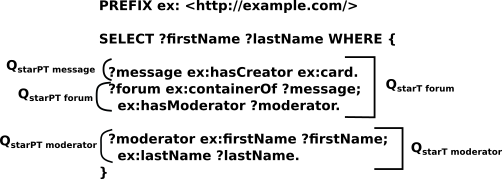
\includegraphics[width=0.8\textwidth]{figure/q_star.png}
   \caption{
      Representation of tree star patterns.
      In red the tree star patterns are presented and in black the partial tree star patterns.
    }
    \label{fig:q_star}
\end{figure}

\begin{definition}[Tree Star Pattern]\label{def:starPattern}
   We define a star pattern $Q_{star}$ as a set of $tp \in Q$~\cite{Karim2020} with the same subject such that 
   given a builder function 
   \begin{equation}
       BQ_{star}(s) = \{tp_i \in Q| S(tp_i) = s\}
   \end{equation}
   with $s \in \mathcal{I} \cup \mathcal{B} \cup \mathcal{V}$ then $Q_{star_s} = BQ_{star}(s)$.
   We define a tree star pattern $Q_{starT}$ as the union between a root star pattern $Q_{star_s}$
   and the star patterns having as subject term an object term of another star pattern in $Q_{starT}$.
   We define a function 
   $O_{star}: q \in Q \rightarrow  \mathcal{I} \cup \mathcal{B} \cup \mathcal{V}$
   that returns every non-literal object terms of a star pattern.

   We then define $Q_{starT}$ given a  set of partial tree star patterns $Q_{starPT}$
   \begin{equation}
       Q_{starT} = \bigcup_{q \in Q_{starPT}} q
   \end{equation}
   where $Q_{starPT}$ is formed with a root $Q_{star_s}$ by

   \begin{equation}
           Q_{starPT_i} =
       \begin{cases}
           \{Q_{star_s}\} & \text{if } i = 1 \\
           \{BQ_{star}(o)| o \in \bigcup\limits_{q \in Q_{starPT_{i-1}}} O_{star}(q)\} & \text{if } i>1
       \end{cases}
   \end{equation}

   We also define a function  
   $S_{star}: q \rightarrow  \mathcal{I} \cup \mathcal{B} \cup \mathcal{V}$
   returning the subjects of the $Q_{starPT_i}$ of a $Q_{starT}$.

   We propose a similar definition for the context of KGs where we replace the query $Q$ by a KG $G$ and where the terms 
   cannot be a $v \in \mathcal{V}$. 
   We denote this structure a tree star.
   
\end{definition}

The construction and maintenance of shape indexes are beyond the scope of this work.
However, we believe they require less effort than void descriptions~\cite{Boehm2011}, which have already been used for query optimization~\cite{Montoya2017}, albeit not in the context of LTQP.
RDF data shapes can be either prescriptive or descriptive.
For shape indexes with descriptive shapes, automatic RDF data shape generation methods~\cite{fernandez2023extracting} could facilitate their creation.
Entries in shape indexes correspond to sets of IRIs, which could be structured using URI templates, thereby reducing the need for exhaustive redefinition.
For prescriptive shapes, contributions in shape-based data integration~\cite{LabraGayo2023} could help prevent the generation of invalid data sources.


\subsection{Link Pruning Using Shape Indexes}\label{sec:sourceSelection}

In this section we make the link between the shape index and link pruning in LTQP.
A DKG exposing a shape index provides a query engine with the opportunity to reduce its search domain by knowing which resources are query-relevant.
More formally, instead of traversing the whole subweb $D$ associated with a shape index, the engine will traverse a subweb $d \subseteq D$, ignoring the knowable query-irrelevant sources.
The concept of composite reachability criteria allows us to ignore certain sources during traversal based on the knowledge acquired during traversal.
Our approach involves dynamically constructing new reachability criteria during traversal by adding pruning critera as we discover and analyze shape indexes.
These criteria are designed so that, they will always produce the same completeness of results as the one that was defined at the beginning of the traversal.

\iffalse
\rt{I still think introducing time here is a really bad idea. I'm almost certain that reviewers will shoot the paper down because of this. In the formalization, let's just assume prior knowledge of all shape indexes and corresponding reachability criteria. Combining them during query execution is an implementation detail.}
More formally, let us introduce time $t$ as a factor for our reachability criteria $C_t$.
The query execution begins with an initial reachability criterion $C_0$.
At any time $t$, Equation~\ref{eq:evalQueryStructuralAssumption} must hold if we consider $C_t = C_{t+1} = C_{t+2} \dots = C_{tf}$ until the end of the execution $tf$, given that $G^{\prime}$ is produced using $C_0$.
\fi
The initial criterion $C_0$ must include a discovery reachability criterion $cd_{\text{shape index}}$ that leads to a shape index document.
After dereferencing a shape index $SI_i$ the query engine creates a set of links $IRI_p$, which contains the links that must be pruned.
The links to prune are determined by evaluating the shape index to identify the set of IRIs that are not query-relevant such that Equation~\ref{eq:evalQueryStructuralAssumption}, given that $G^{\prime}$ is produced using $C_0$.
This is achieved by performing a query-shape containment check ($\sqsubseteq_{qs}$), as defined in Section~\ref{sec:containment}.
We define
$IRI_p = \{ \bigcup_{iri \in SI_i(s_j)} iri | B \sqsubseteq_{qs}  s_j = \mathrm{false}, s_j \in \text{dom}(SI_i) \}$.
From this sets of links we define a pruning reachability criteria;
\begin{equation}
       cp_{si}(t, iri, B) = iri \notin IRI_p
\end{equation}
The new reachability $C^{\prime\prime}_i$ is created by taking the $Cd$ and $Cp$ of $C^{\prime\prime}_{i-1}$ and adding
and $cp_{si}$ to $Cp$.

This approach has two main limitations.
First, it assumes that data providers maintain up-to-date shape indexes.
If the indexes are outdated, results may be incomplete.
A similar criticism could be made against the method exploiting void descriptions~\cite{Montoya2017}.
Furthermore, if the shape query containment check requires dereferencing all documents, the operation becomes effectively useless and may increase query execution time.
Second, the approach does not account for cases where querying irrelevant documents could lead to relevant ones based on additional reachability criteria.
Addressing this during the containment check would require translating these criteria into queries and incorporating them into the evaluation process.
However, this is beyond the scope of this paper.

\subsection{Query Shape Containment}\label{sec:containment}

We consider determining if a source is query-relevant a \emph{query-shape containment} problem.
The understanding of this problem is similar to the classic query containment problem.
Query containment determines if a query can be answered from the answer of another query, that we denote container query, independent to the database or KG~\cite{afariQCE, Spasi2023}.
In our version of query-shape containment, we want to determine if a tree star pattern from a query can be answered by any sources respecting a specific shape.

Intuitively shapes expressions can be translated into segments of queries~\cite{delva2023}.
Furthermore it is a common approach for shape validation over an RDF graph is to convert shapes into SPARQL queries~\cite{labragayo2017validatingdescribinglinkeddata, Corman2019,Prestamo2023, spapeExpressionConvert}.~\sepfootnote{sf:recursiveShape}
We refer to this transformation of a shape $s$ as $T(s)$ producing a query $Q_s$.
We consider shapes with open world assumption to always represent queries that retrieve entire KGs, if we ignore negative statement such has KG validating this shape does not have this property.
This is because, under the open-world assumption, a shape defines the minimum constraints of a graph.
With this transformation query-shape containment becomes similar to query containment problems.

Query containment may intuitively seem unsuitable for dynamic reachability due to its NP-complete time complexity~\cite{Spasi2023}.
However, this complexity depends on the size of the queries, which are typically small in practise~\cite{Doan2012}; we do not expect in most cases queries containing thousands or millions of triple patterns~\cite{Bonifati2019}.
Additionally, practical use cases can often leverage polynomial-time algorithms~\cite{Doan2012}.
In our context, the container query adheres to a tree-star pattern template structure, where predicates are always IRIs.
This structure arises because shapes predominantly describe predicate terms and object terms and are isomorphic to the specific KG.
By exploiting this structure, it is possible to design an algorithm with polynomial time complexity.

We consider that a query $Q$ is contained in a shape $S$, denoted as $Q \sqsubseteq_{qs} S$, if a tree star pattern in $Q$ is contained in $Q_s = T(S)$. 
For a tree star pattern to be contained, we need to consider the two parts of $Q = Q_{\text{body}} \cup Q_{\text{unions}}$ and ignore other forms of queries.
$Q_{\text{body}}$ is the Basic Graph Pattern (BGP) of the query, and $Q_{\text{unions}} = \bigcup Q_u$ represents the Union Graph Patterns (UGP), where $Q_u = q_0 \cup q_1 \cup q_2 \dots \cup q_n$.
We assume that $q_i$ are not union statement.
A tree star pattern $Q_{\text{starT}_i}$ is contained in $Q_s$ if its segment in $Q_{\text{body}}$ is contained in $Q_s$, and if its segment in at least one $q_i$ in each $Q_u$ is contained in $Q_s$. 
If $Q_{\text{starT}_i}$ is not part of any $Q_u$, then $Q_u$ is ignored.

For the simplicity of the formalization we ignore other SPARQL operators such has \texttt{GROUP BY} and Filter expressions,
however given query-shape containment is transformed into query containment problem there are methods in the litterature to handle a more complete SPARQL fragment~\cite{Spasi2023}.

\iffalse
\rt{I would not mention everything after this, and instead at the start of this paragraph say that for simplicity of this formalization, we focus on just BGPs of triple patterns and unions.}
In our containment problem, we ignore \texttt{GROUP BY} segments.
We make this choice because, in the context of shape queries, \texttt{GROUP BY} is primarily used to set a cardinality, and we are not attempting to identify sources that can fully answer specific segments of a query. 
Instead, our goal is to disregard data sources that are irrelevant to the query, given the constraints imposed by the shape index. 
Discriminating based on cardinalities could potentially affect query results.
Additionally, this article does not consider filter expressions, as they can significantly increase the complexity of the problem.
Moreover, "false" negatives do not impact the correctness of our approach. \rt{But this is important to mention indeed! But needs some more elaboration on the fact that doing more (useless) requests is not a problem.}
However, incorporating filter expressions into future work would be an interesting direction to explore.
\fi
% https://en.wikipedia.org/wiki/Master_theorem_(analysis_of_algorithms)
\begin{algorithm}[h]
   \caption{Determine if a tree star pattern is contained ($isContain_{\text{Tree star}}$)}\label{alg:containmentTree}
   \begin{algorithmic}
      \REQUIRE  $Q_{star}$, $Q_{starT_i}$, $Q_s = Q_{s\text{body}} \cup Q_{s\text{unions}}$ and $Eval_{star}$
      \ENSURE \TRUE $ $ or \FALSE $ $ whether the tree star pattern is contained in the shape

      \IF{$S_{star}(Q_{star}) \in Eval_{star}$}
         \RETURN \TRUE
      \ENDIF 

      \FORALL{$tp \in Q_{star}$} % O(n_star)
         \IF{\NOT $match(tp, Q_{s\text{body}})$}
            \STATE $hasOnePath \gets $ \FALSE
            \FORALL{$q_{us} \in Q_{s\text{unions}}$}
               \IF{$isContain_{\text{Tree star}}(Q_{star}, Q_{starT_i}, q_{us}, Eval_{star})$}
                  \STATE $hasOnePath \gets $ \TRUE
               \ENDIF
            \ENDFOR
            \IF{\NOT $hasOnePath$}
               \RETURN \FALSE
            \ENDIF
         \ELSE
            %eval nested
            \IF{$O(tp) \in  S_{star}(Q_{starT_i})$}
               \IF{\NOT $isContain_{\text{Tree star}}(Q_{star_{O(tp)}} \in Q_{starT_i}, Q_{starT_i}, Q_s, Eval_{star})$}
                  \RETURN \FALSE
               \ENDIF
            \ENDIF
            %
         \ENDIF
      \ENDFOR

      \STATE $Eval_{star} \gets Eval_{star} \cup S_{star}(Q_{star})$
      \RETURN \TRUE
   \end{algorithmic}
\end{algorithm}


We define the function $isContain_{\text{Tree star}}$ in Algorithm~\ref{alg:containmentTree} to evaluate whether a tree star pattern with a root star pattern $Q_{star_i}$ from $Q_{starT_i}$ is contained in $Q_s$. 
The algorithm also takes a set $Eval_{star}$ to track which partial tree stars have already been evaluated.
The algorithm works by examining each triple pattern in the root star pattern $Q_{star_i}$ and checking if an equivalent triple pattern (ignoring the variable names) can be found in the BGP of $Q_s$ using the $match$ function.
If the triple pattern cannot be found in the BGP, the algorithm then looks into the UGPs of $Q_s$. 
Since we assume that the union statements are not nested, this limits the number of recursive calls.
If an equivalent triple pattern is found, the algorithm checks whether the object of the triple pattern is the subject of a partial tree star pattern in $Q_{starT_i}$.
If it is, the algorithm recursively applies the same procedure to this partial tree star pattern as $Q_{star_i}$.
To avoid cycles and redundant evaluations when processing the object of the star patterns, we maintain a set of evaluated subjects in $Eval_{star}$.
We notice that the complexity of Algorithm~\ref{alg:containmentTree} is $O( n_o \times n_{tp}^2 \times n_{sunion}^2)$
where $n_{tp}$ is the number of triple patterns of $Q_{star_i}$, $n_{sunion}$ the number of UGP in $Q_s$ and $n_o$ the number of object term in $Q_{starT_i}$.
To solve $Q \sqsubseteq_{qs} S$, we need to consider the number of tree stars from the BGP with their number of segments in the UGP and the number of BGPs in the UGPs.
This operation results again in a polynomial time complexity algorithm.
%To solve $Q \sqsubseteq_{qs} S$, we need to consider the $n_{starT}$ tree star from the BGP with their $n_{starTu}$ segment in the UGP and $n_{starTui}$ BGP in the UGP.
%This operation results in a polynomial time complexity of $O(n_o \times n_{tp}^2 \times n_{union}^2 \times n_{starT} \times n_{starTu} \times n_{starTui})$.
%In the \nameref{sec:appendix} Algorithm~\ref{alg:containment} present the full resolution to evaluate each tree star pattern.
